\documentclass[12pt]{article}
\usepackage[margin=1in]{geometry}
\usepackage{amsmath}
\usepackage{graphicx}
\usepackage{setspace}
\usepackage{subcaption}
\usepackage{listings}
\usepackage[italicdiff]{physics}
\usepackage{natbib}
\usepackage{epstopdf}
\lstset{breaklines=true, tabsize = 3}

\author{Jonathan Bunton}
\title{Analysis of the Ising Model with a\\ Metropolis Monte-Carlo Simulation}
\date{\today}

\begin{document}
\maketitle
\onehalfspacing
\begin{abstract}
Different classes of magnetic materials experience a variety of different effects on the atomic level, which often scale into noticeable effects on the macro scale.  These effects directly impact the material's energy, causing certain quantum mechanical spin states to be more favorable than others as governed by the material's partition function.  One of the simplest methods of analyzing these effects on a larger scale is through the Ising model, which identifies the presence of phase transitions for magnetic materials dimensions two or higher. \cite{isingmodel}  The Hamiltonian for these materials in the Ising model is defined by:
\begin{align}
H &= -\mu_B\sum_i s_i - \mu_B^2J\sum_{neighbors}s_i s_j.
\label{H}
\end{align}

This particular paper analyzes the Ising model through the Metropolis Monte-Carlo algorithm, and compares three different material types: ferromagnetic, antiferromagnetic, and paramagnetic.  Each of these material types is under an applied magnetic field $B$ and held at a temperature $T$.  The simulation of these materials reveals temperature-dependent transitions in behavior, which occur at the Curie temperature $T_C$ and the N\'{e}el temperature $T_N$.
\end{abstract}
\section*{Results}
The Monte Carlo algorithm is a useful tool in this analysis as it allows for the iterative calculation of averages with sampling occurring over a specified distribution. \cite{montecarlo} In this particular paper, a $10\times10\times10$ lattice of iron atoms is examined under a range of temperatures and applied magnetic fields.  Each individual point was run through $100,000$ Monte-Carlo sweeps in an effort to smooth graphs and make averages as accurate as possible, resulting in reliable results.

\subsection*{Ferromagnetism}
A ferromagnet is defined by its characteristic strong interactions between neighboring spins as a result of the exchange interaction.  For this simulation, we use an exchange coefficient $J = 2.0929E25 > 0$ to ensure the exchange forces were high and tend to align spins with each other. \cite{magnettypes, fromjesse}

%Ferromagnet 3D scatters
\begin{figure}[!h]
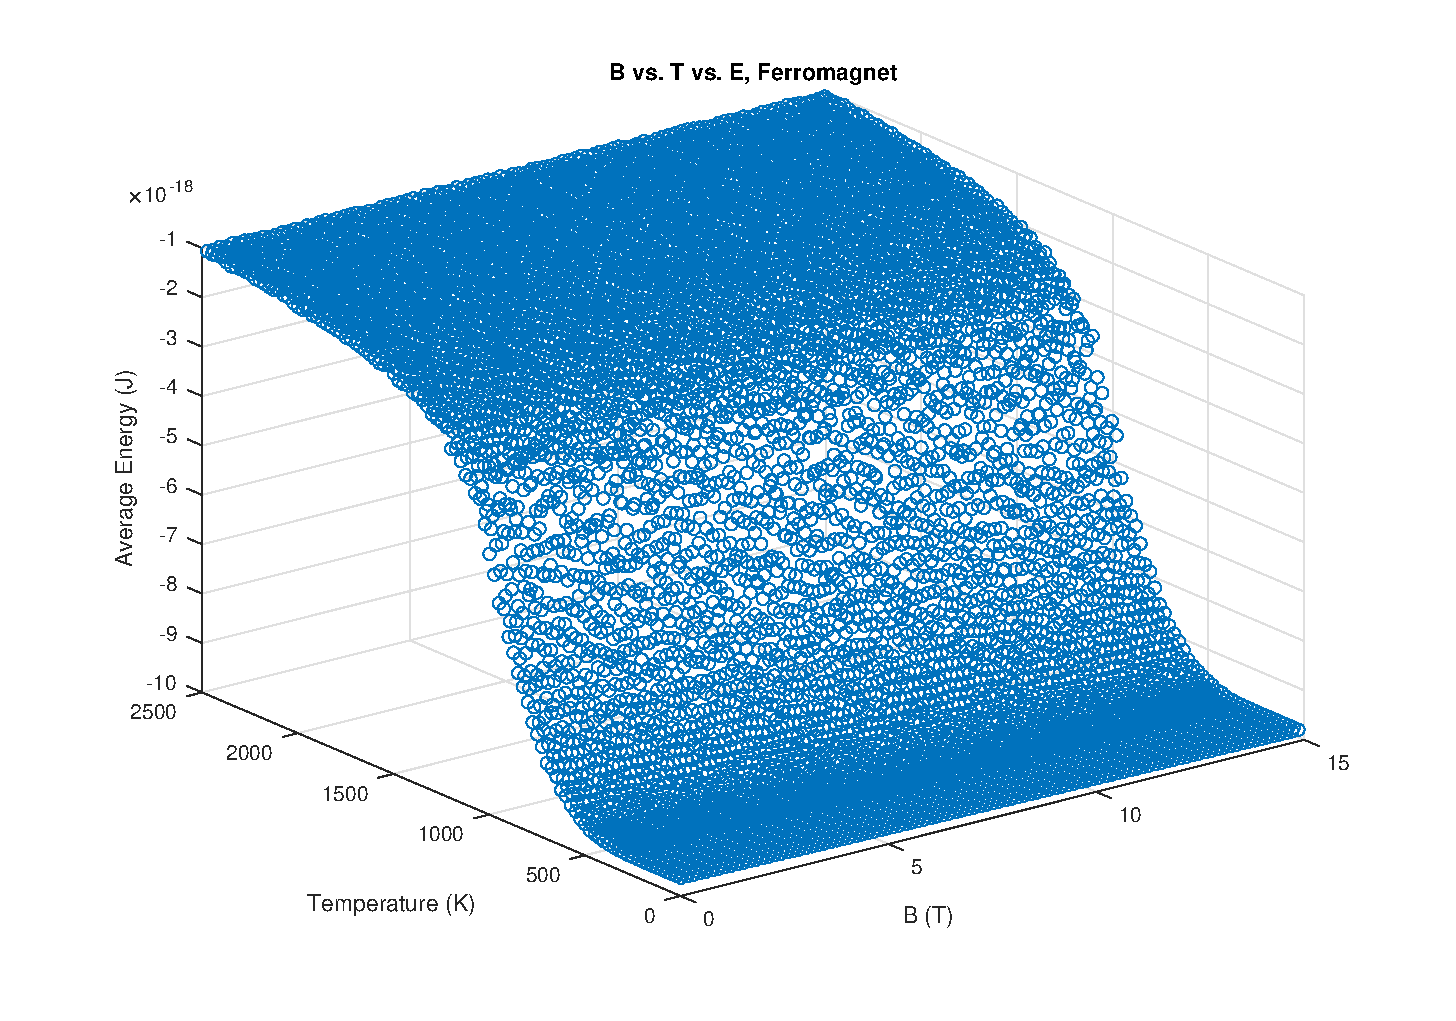
\includegraphics[width=\linewidth]{./Ferrographs/ferroEsurf.eps}
\caption{A 3D scatter plot of average energy as a function of applied magnetic field $B$ and temperature $T$.}
\label{ferroEsurf}
\end{figure}
The generated data shown in fig. \ref{ferroEsurf} shows a clear ``S" shape as temperature is increased, consistent through all magnetic field values.  This trend indicates that as temperature is increased, the average energy of the lattice also increases, but only past a particular threshold.

\begin{figure}[!h]
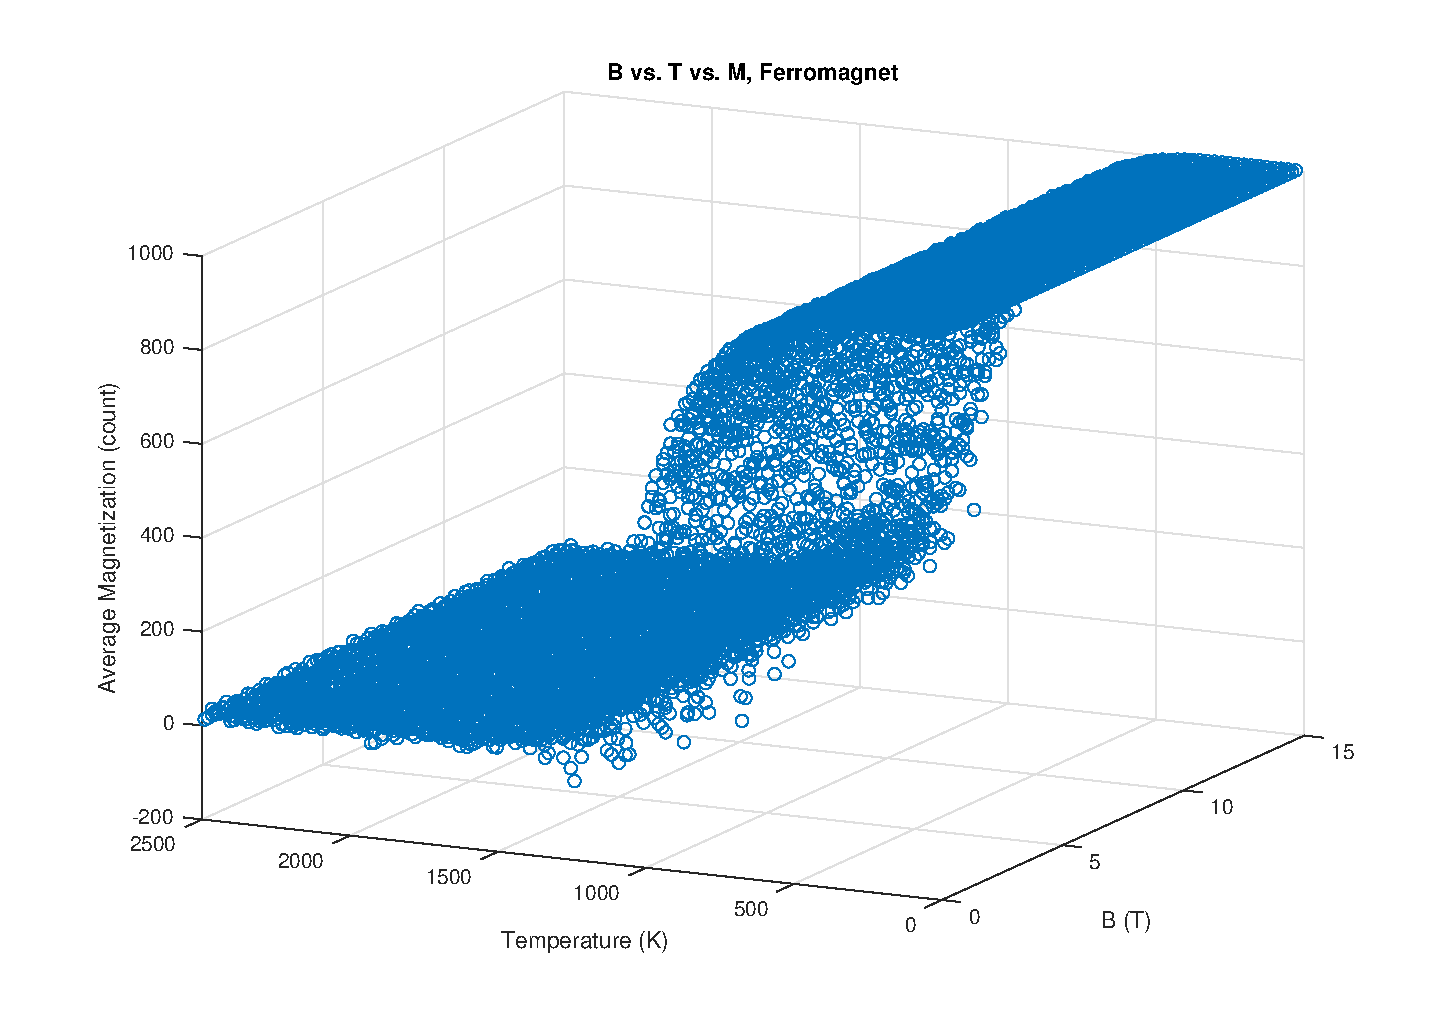
\includegraphics[width=\linewidth]{./Ferrographs/ferroMsurf.eps}
\caption{A 3D scatter plot of average magnetization as a function of applied magnetic field $B$ and temperature $T$ for a ferromagnetic material.}
\label{ferroMsurf}
\end{figure}
Conversely to \ref{ferroEsurf}, the plot of average magnetization shows an opposite trend, where past a similar temperature threshold the average drops to zero.

%Ferromagnet T-dependent plots
\begin{figure}[!h]
\begin{subfigure}{0.5\textwidth}
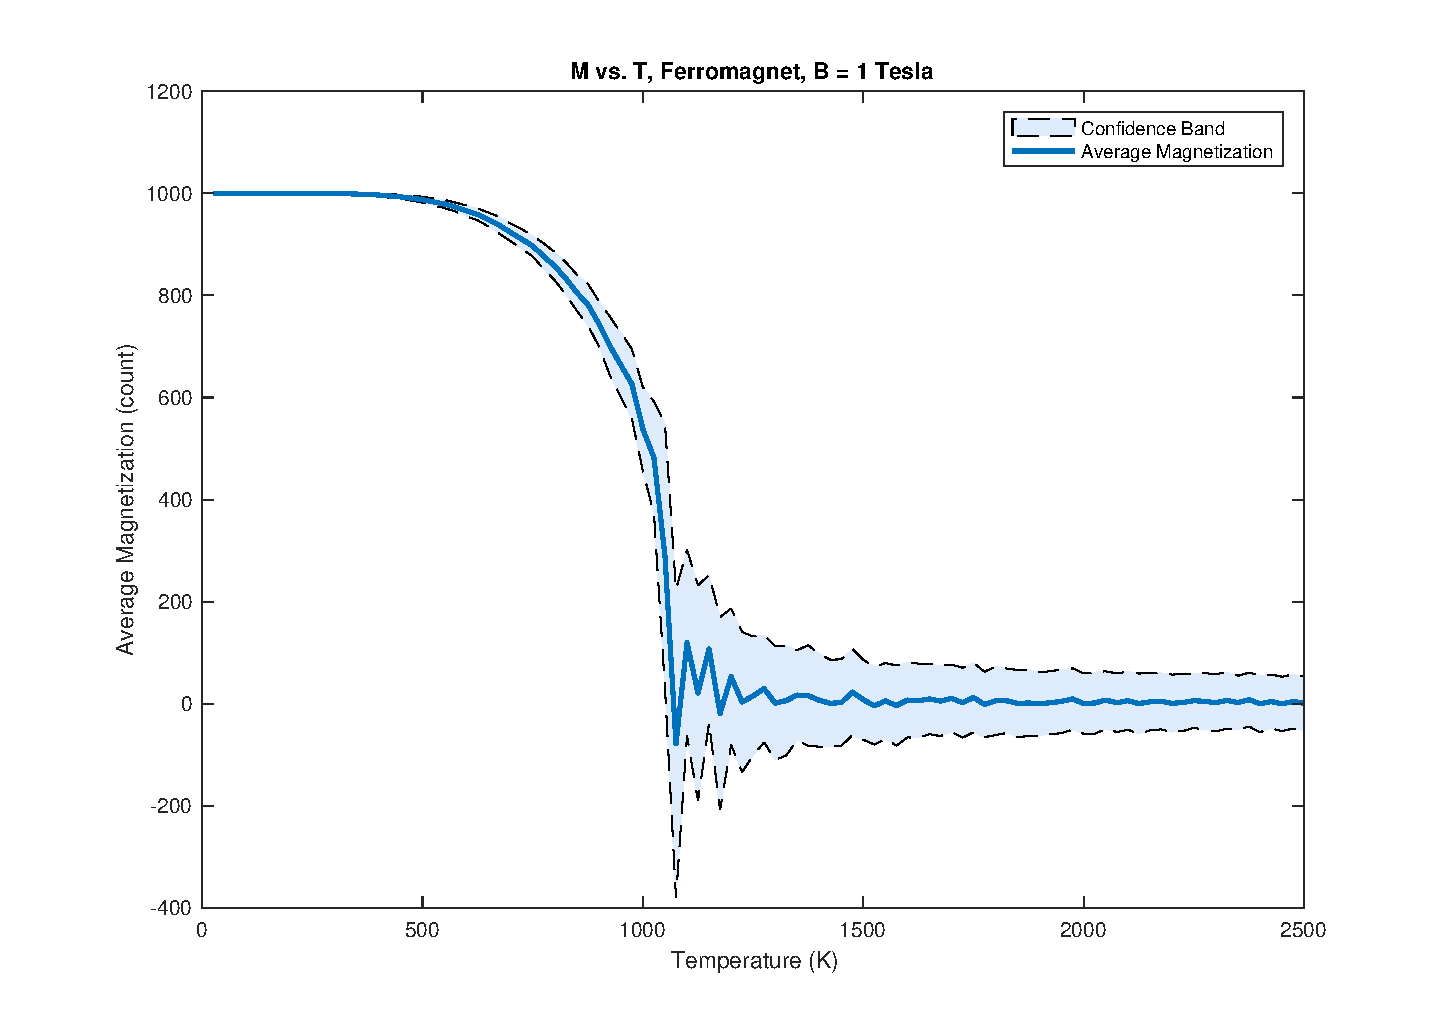
\includegraphics[width=\linewidth]{./Ferrographs/ferroMvsT.eps}
\caption{\label{ferroMvsT}}
\end{subfigure}
\begin{subfigure}{0.5\textwidth}
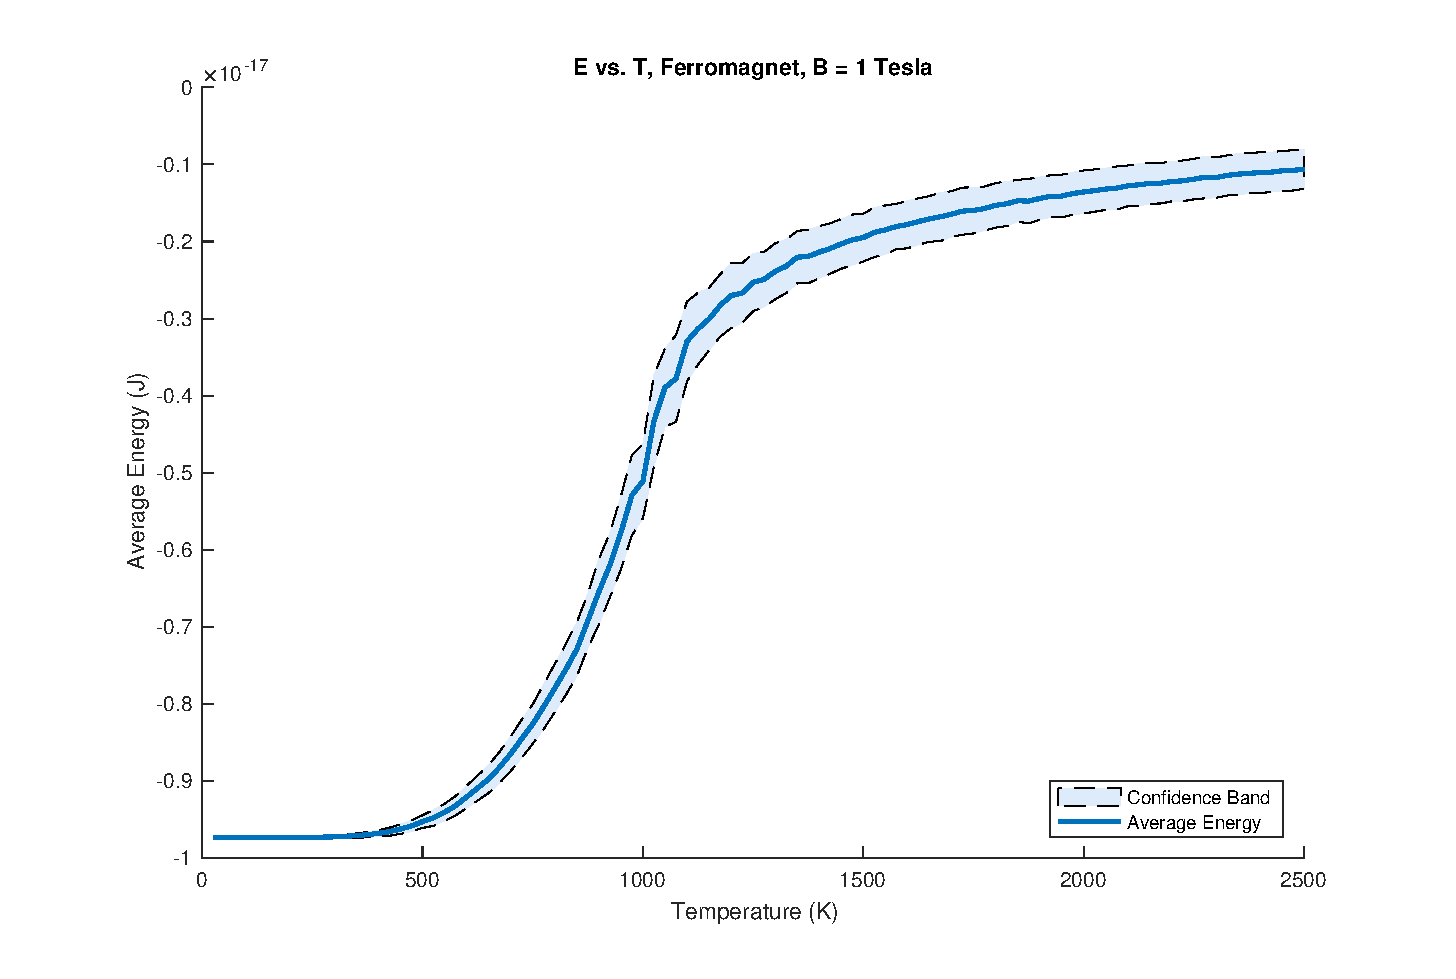
\includegraphics[width=\linewidth]{./Ferrographs/ferroEvsT.eps}
\caption{\label{ferroEvsT}}
\end{subfigure}
\caption{Plots of (a) average magnetization and (b) average energy as a function of temperature.  These plots were produced using an applied magnetic field $B = 1$ T for a ferromagnetic material.} 
\end{figure} 
Analyzing individual strips of this plot in figs. \ref{ferroMvsT} and \ref{ferroEvsT} shows the threshold temperature for the trends to be around $T_C = 1000$ K.  $T_C$ is the Curie temperature, above which a ferromagnetic material has access to enough thermal energy to overcome the strong exchange forces holding its magnetization in place.  In other words, above $T_C$ the ferromagnet behaves as a paramagnet. \cite{magnettypes, fromjesse}
%Ferromagnet B-dependent plots
\begin{figure}[!h]
\begin{subfigure}{0.5\textwidth}
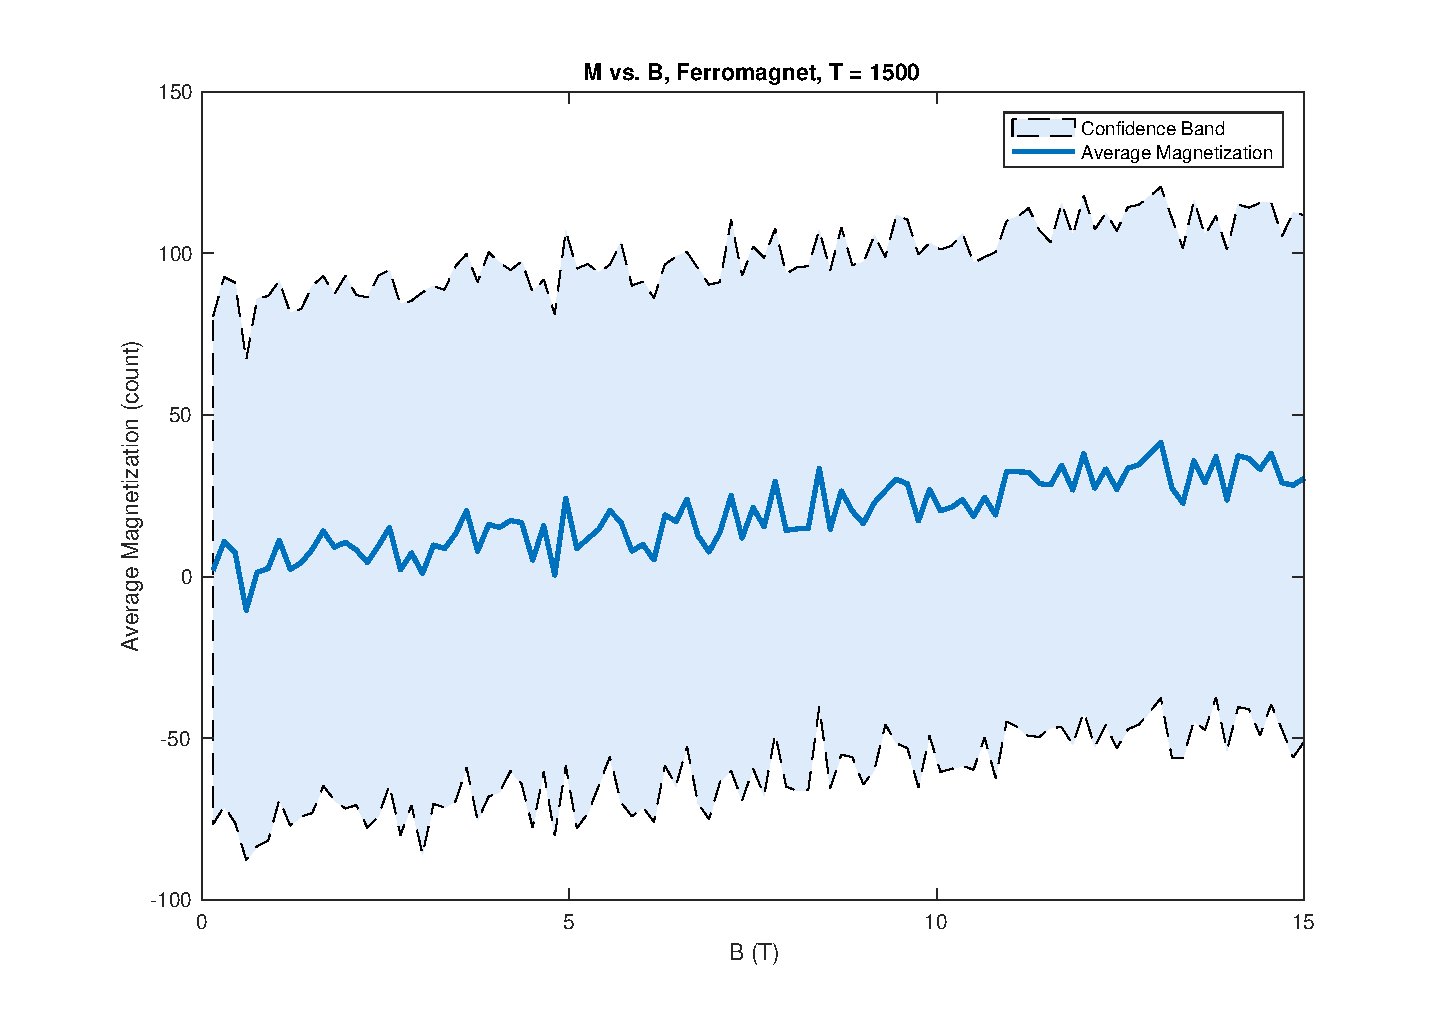
\includegraphics[width=\linewidth]{./Ferrographs/ferroMvsB.eps}
\caption{\label{ferroMvsB}}
\end{subfigure}
\begin{subfigure}{0.5\textwidth}
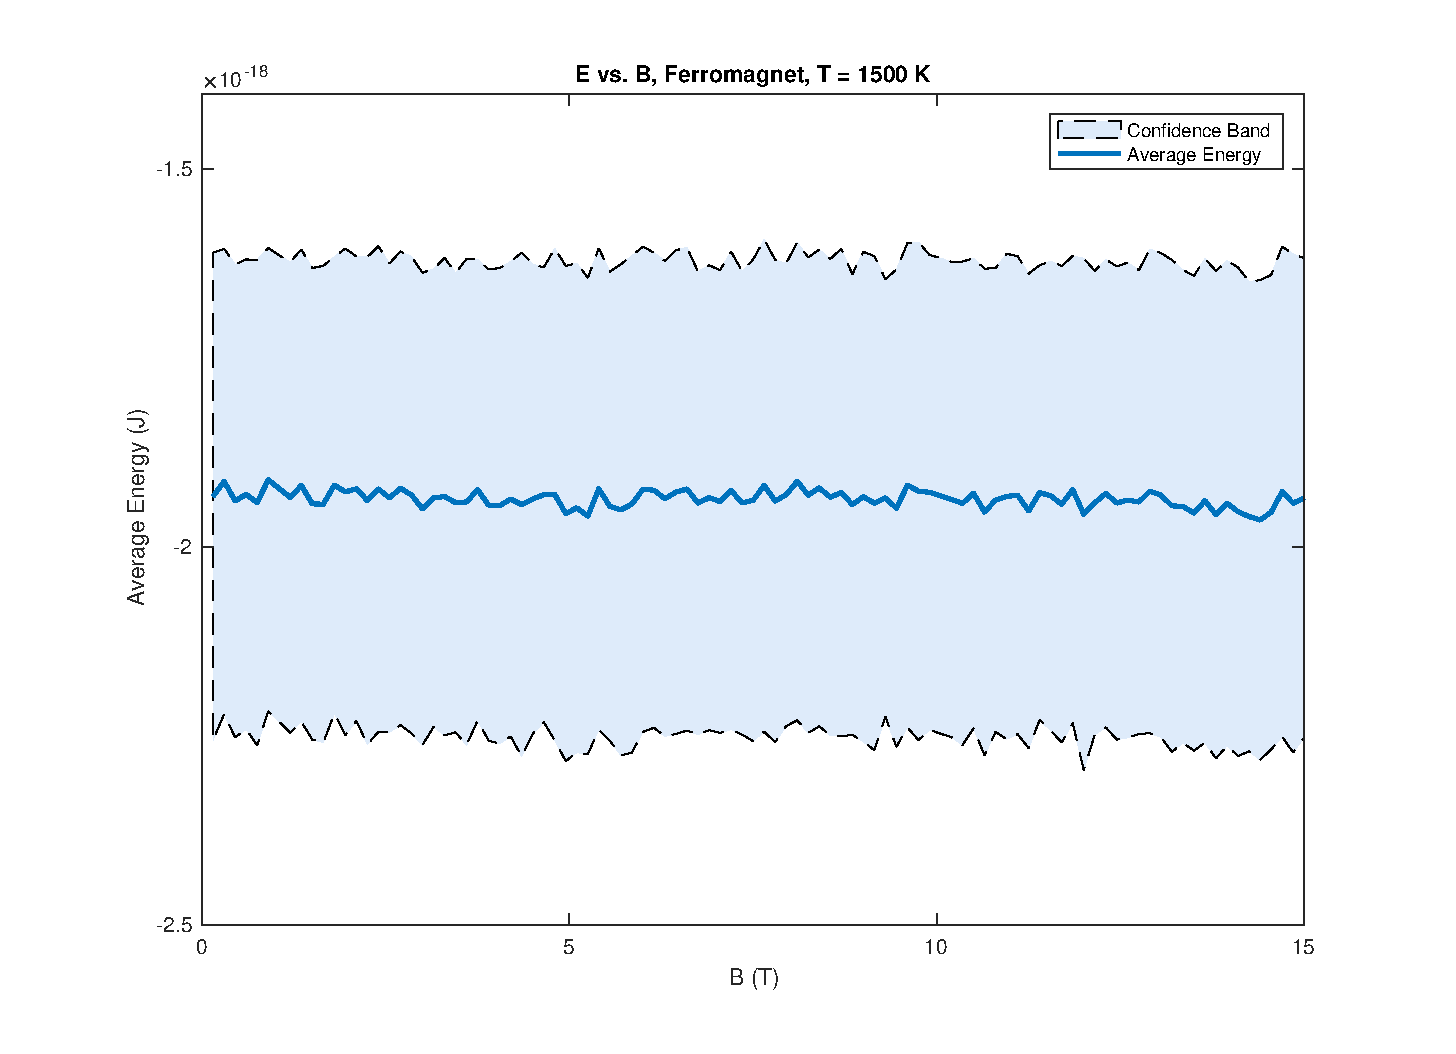
\includegraphics[width=\linewidth]{./Ferrographs/ferroEvsB.eps}
\caption{\label{ferroEvsB}}
\end{subfigure}
\caption{Plots of (a) average magnetization and (b) average energy as a function of applied magnetic field for a ferromagnetic material.  These plots were produced using a temperature of $T = 1500$ K.} 
\end{figure}
The applied magnetic field appears to have a linear effect on the overall magnetization of the ferromagnet when held at $T=1500$ K, as shown in fig. \ref{ferroMvsB}.  This makes sense, as the stronger the applied magnetic field $B$, the more spin states will align parallel.  This effect is weak when compared to the exchange force, which is shown by the small linear slope.  Conversely, the average energy trends slightly downward, which holds with our Hamiltonian (Eq. \ref{H}) stating aligned spin states have lower energy.  However, the system's energy in the ferromagnet is still dominated by the exchange energy, causing $B$ to have a minimal effect.

\subsection*{Antiferromagnetism}
The spin states in an antiferromagnetic material have a lower energy when they are positioned opposite to their neighbors.  Mathematically, this means in our Hamiltonian (Eq. \ref{H}), $J = -2.0929E25 < 0.$ \cite{magnettypes} In order to sample the energies appropriately, the Monte Carlo algorithm is run through an initial set of burn-in sweeps to move towards a lower initial energy.  This lower initial energy avoids unnecessarily oversampling higher energy terms.

%Antiferromagnet 3D scatters
\begin{figure}[!h]
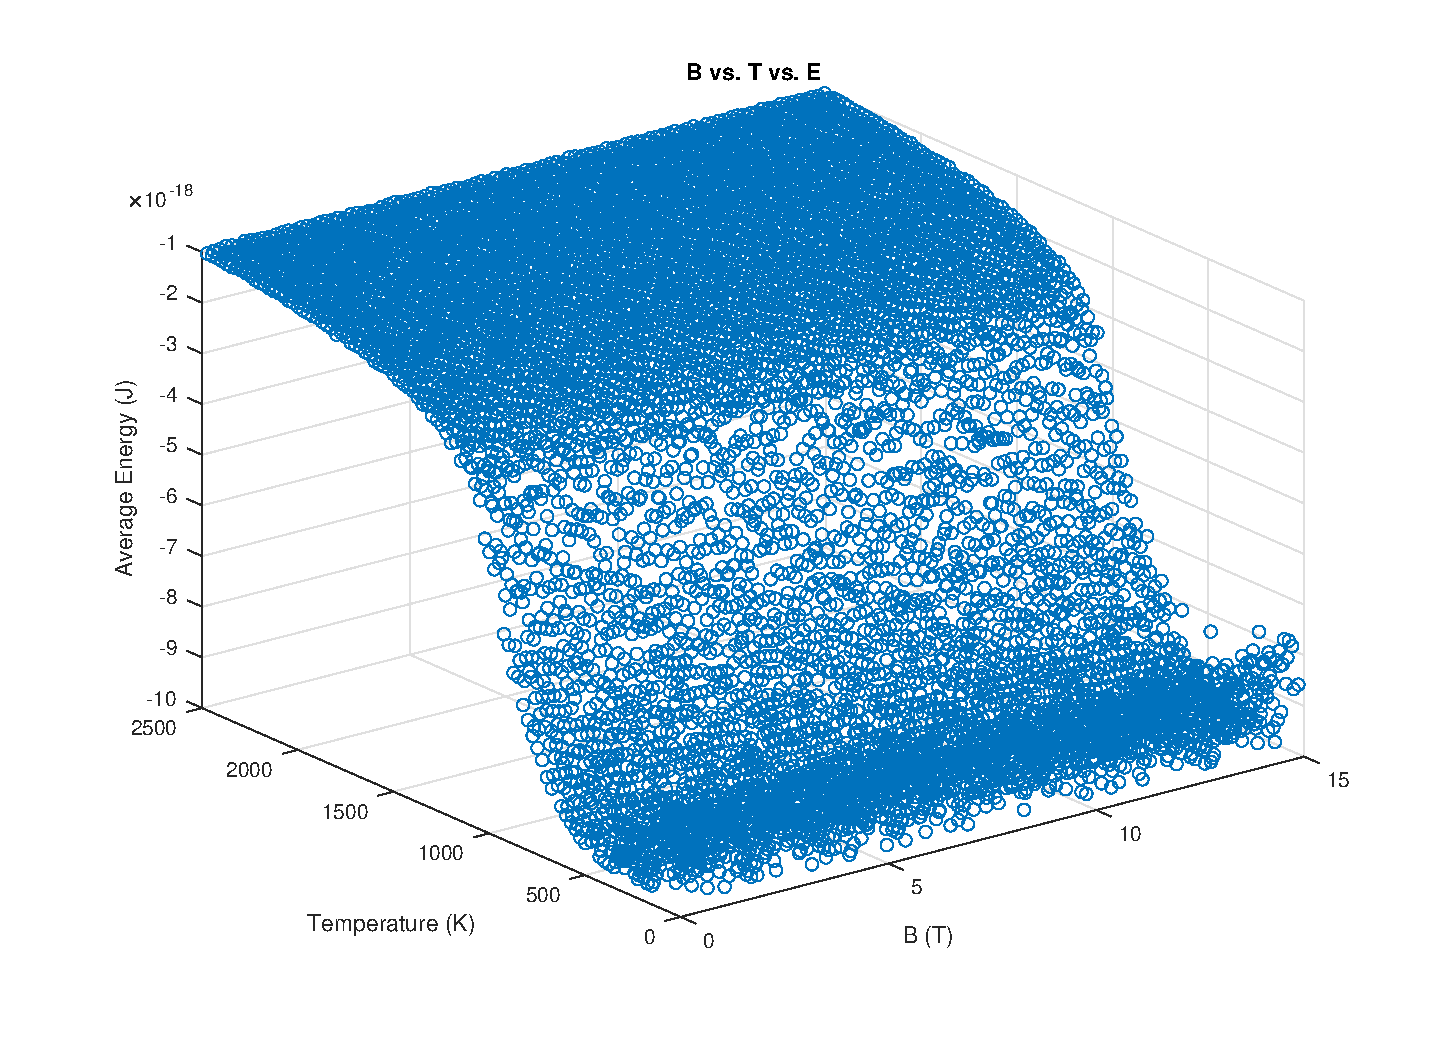
\includegraphics[width=\linewidth]{./Antiferrographs/antiferroEsurf.eps}
\caption{A 3D scatter plot of average energy as a function of applied magnetic field $B$ and temperature for an antiferromagnetic material.}
\label{antiferroEsurf}
\end{figure}
The energy of the antiferromagnetic material (Fig. \ref{antiferroEsurf} appears to behave almost identically to the ferromagnet, where past the threshold of $T_C=1000$K temperature and average energy are positively correlated.  There is also a noteworthy small bump at low temperatures that consistently occurs in calculation. 

\begin{figure}[!h]
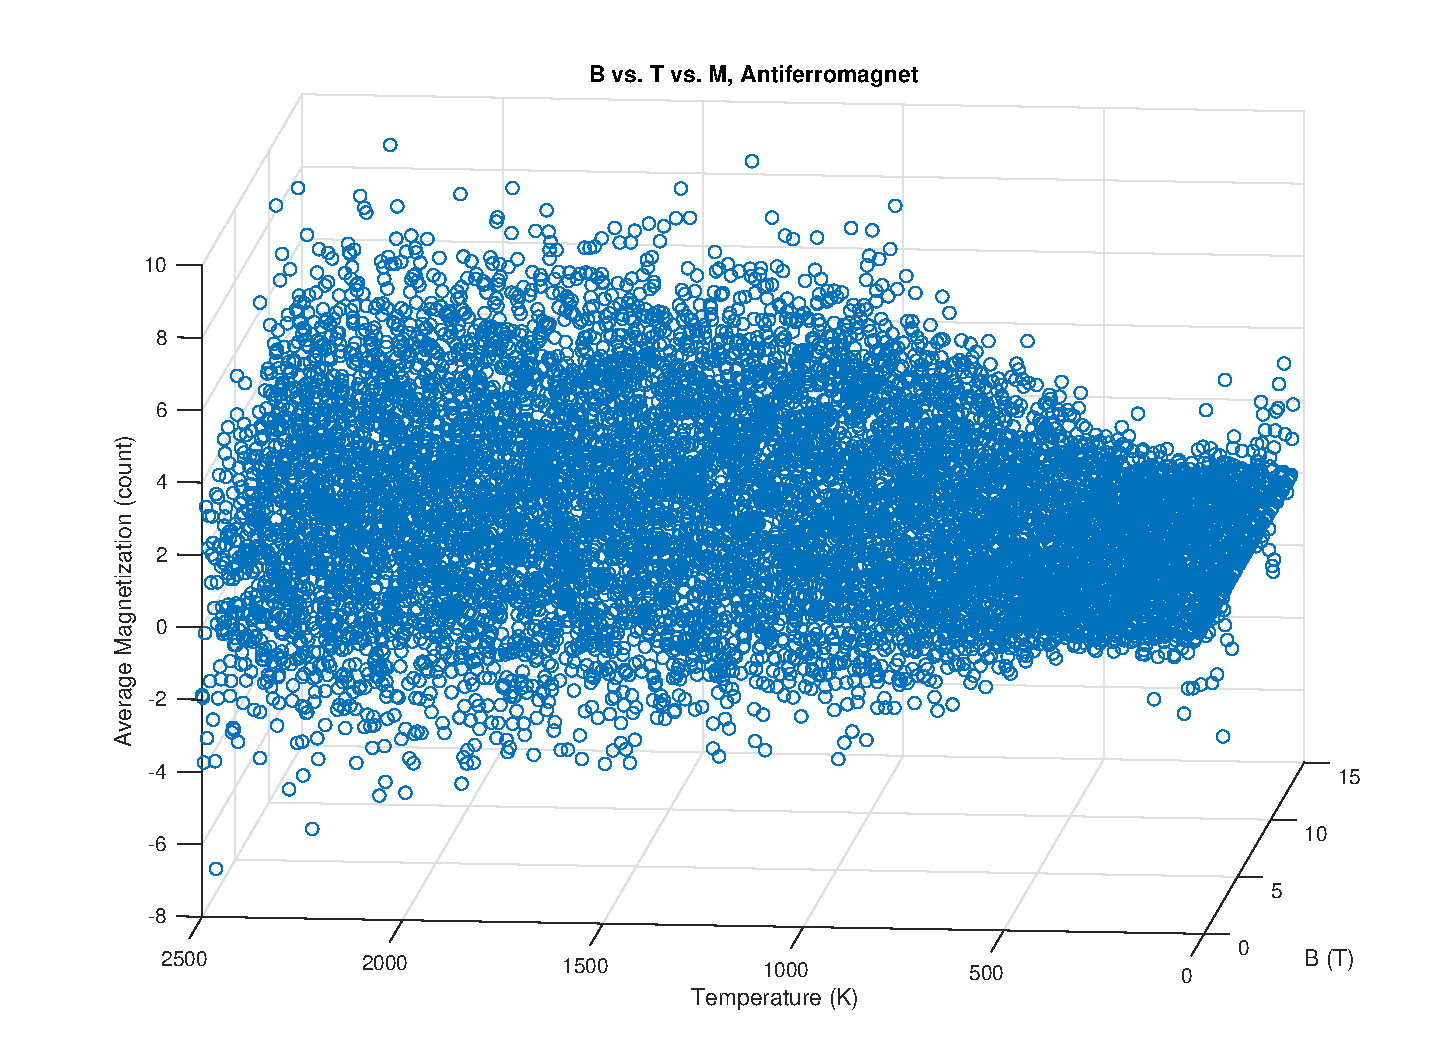
\includegraphics[width=\linewidth]{./Antiferrographs/antiferroMsurf.eps}
\caption{A 3D scatter plot of average magnetization as a function of applied magnetic field $B$ and temperature $T$ for an antiferromagnetic material.}
\label{antiferroMsurf}
\end{figure}
The major difference for the antiferromagnetic case occurs in the calculation of magnetization.  Because the internal spins of the material have a natural tendency to stay oriented opposite each other, the total magnetic moment tends to stay near zero.  As the temperature is increased, there is more energy available to the system, allowing for more probable sampling from states with higher magnetizations.

%Antiferromagnet T-dependent plots
\begin{figure}[!h]
\begin{subfigure}{0.5\textwidth}
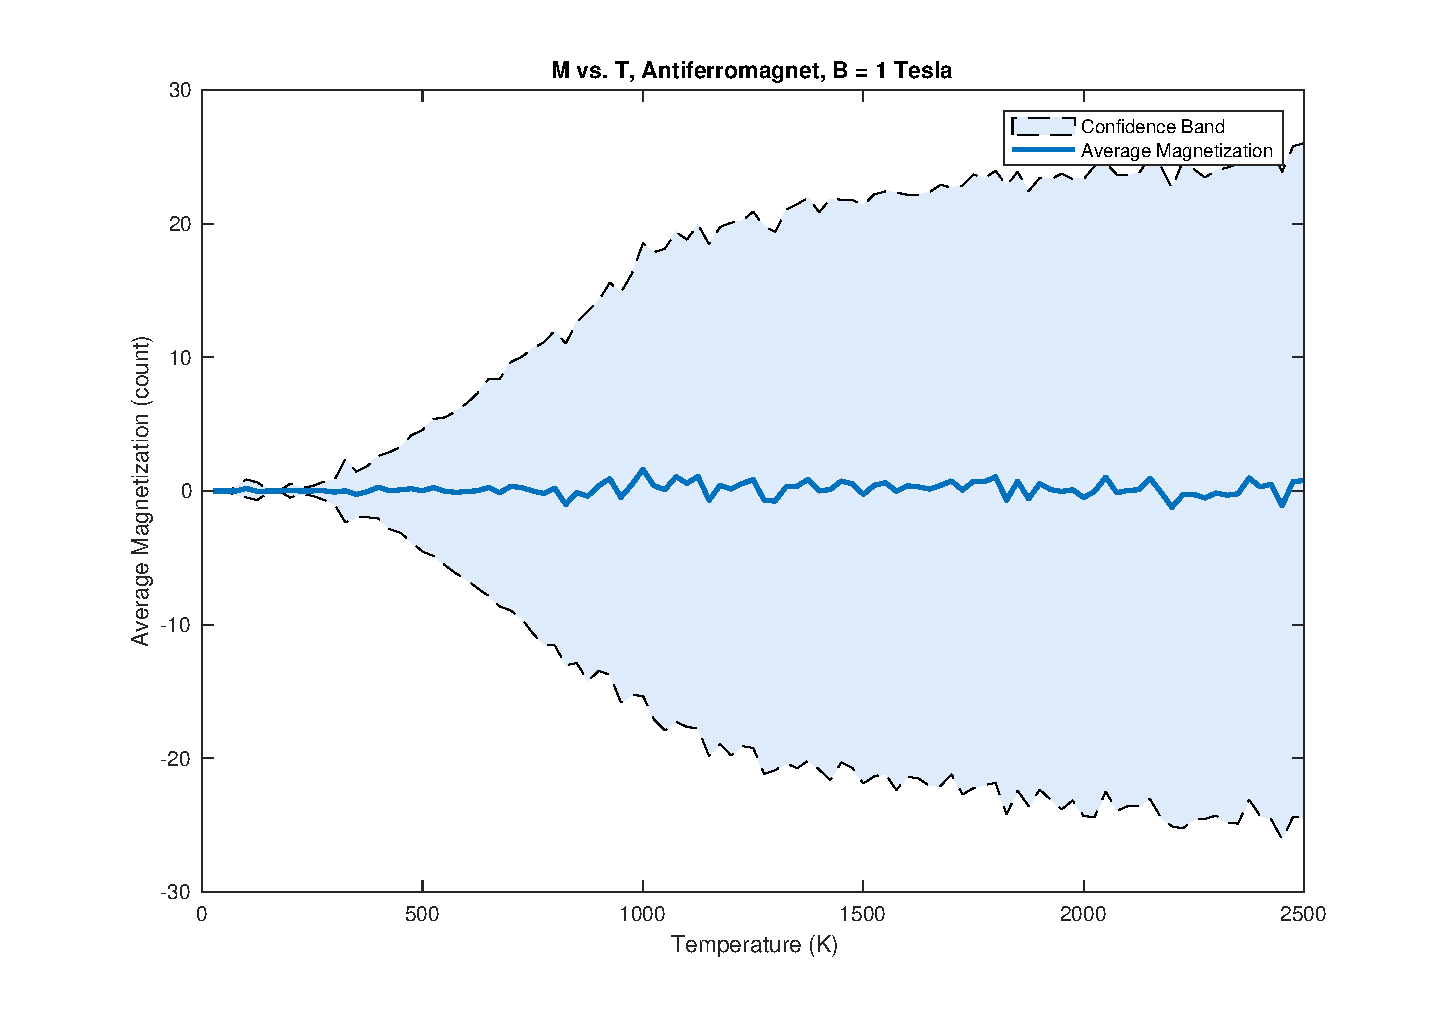
\includegraphics[width=\linewidth]{./Antiferrographs/antiferroMvsT.eps}
\caption{\label{antiferroMvsT}}
\end{subfigure}
\begin{subfigure}{0.5\textwidth}
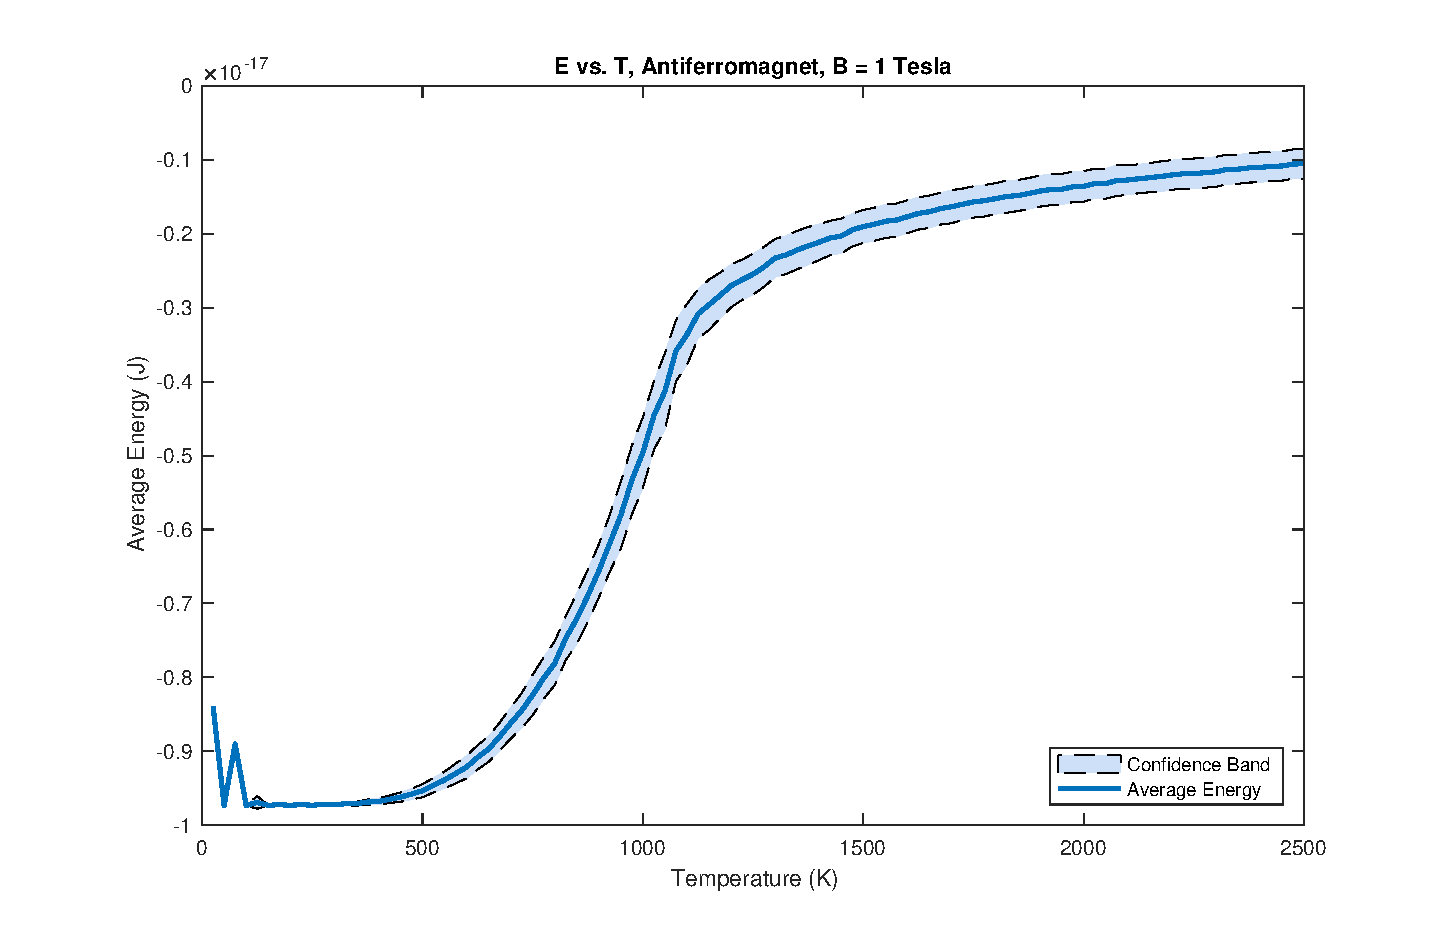
\includegraphics[width=\linewidth]{./Antiferrographs/antiferroEvsT.eps}
\caption{\label{antiferroEvsT}}
\end{subfigure}
\caption{Plots of (a) average magnetization as a function of temperature, and (b) average energy as a function of temperature for an .  These plots were produced using an applied magnetic field $B$ = 1 T.} 
\end{figure} 
The trend shown in our 3D scatter plots is even more evident in figs. \ref{antiferroMvsT} and \ref{antiferroEvsT}.  There is marginal change in the magnetization as the temperature increases, as the randomizing effect of available thermal energy works alongside the antiferromagnetic tendency for spins to oppose each other.  The average energy appears to have the same logistic shape as before, with shifts in the behavior occurring again at approximately $T = 1000$ K.  Above this threshold temperature, the material has enough energy to move more freely against the powerful exchange energy, just as in the ferromagnetic case.  The initial bump in energy occurs at the approximate locaiton for the N\'{e}el temperature, where an antiferromagnetic material begins to behave as a paramagnet. \cite{magnettypes, fromjesse}  This appears to happen in the range $50 < T_N < 100$.

%Antiferromagnet B-dependent plots
\begin{figure}[!h]
\begin{subfigure}{0.5\textwidth}
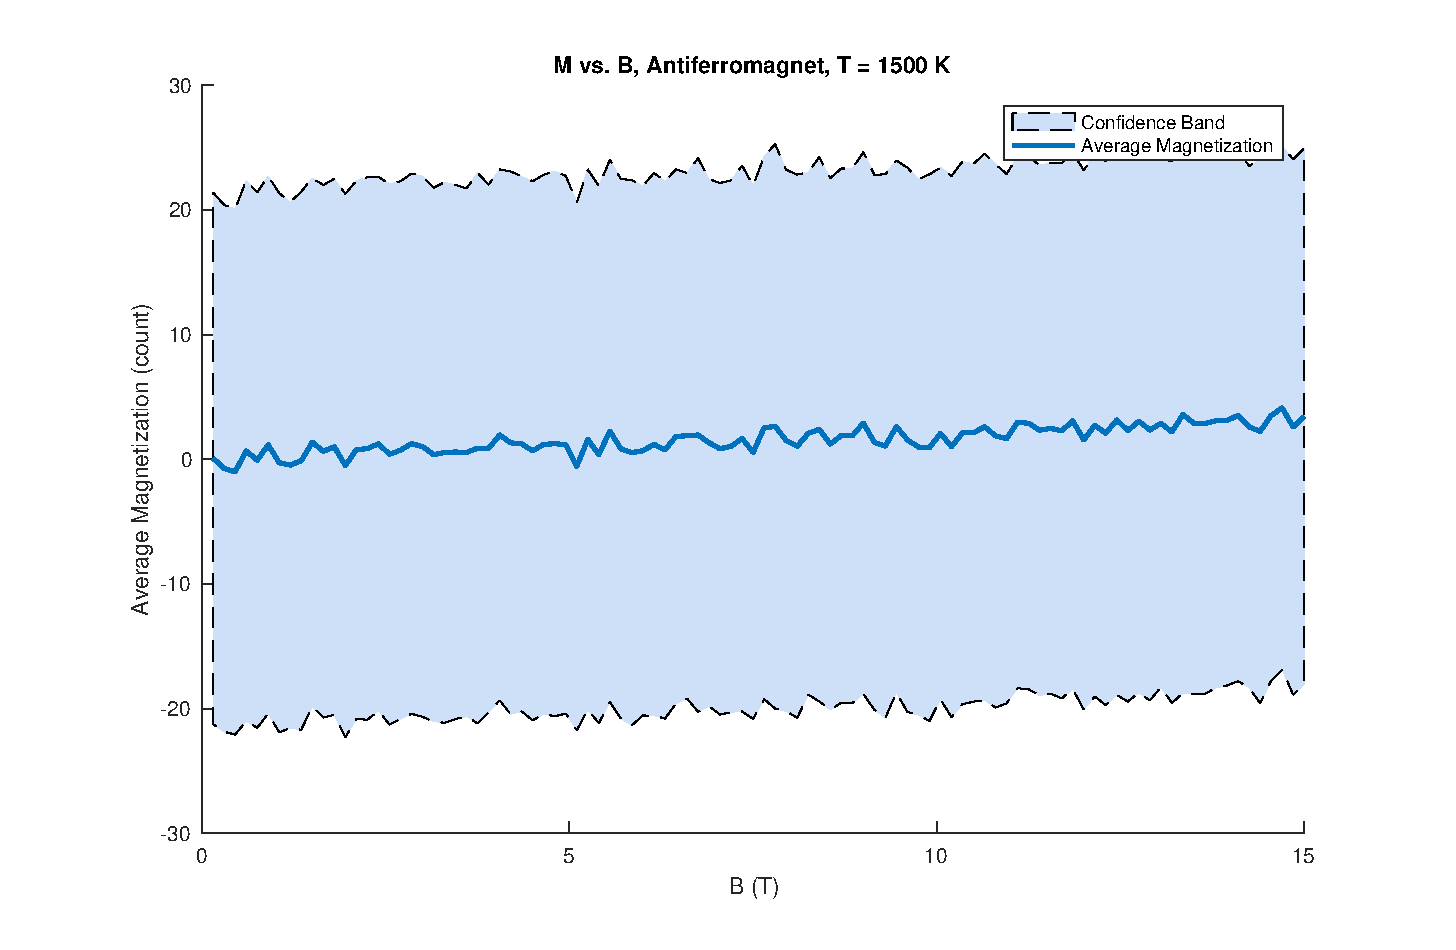
\includegraphics[width=\linewidth]{./Antiferrographs/antiferroMvsB.eps}
\caption{\label{antiferroMvsB}}
\end{subfigure}
\begin{subfigure}{0.5\textwidth}
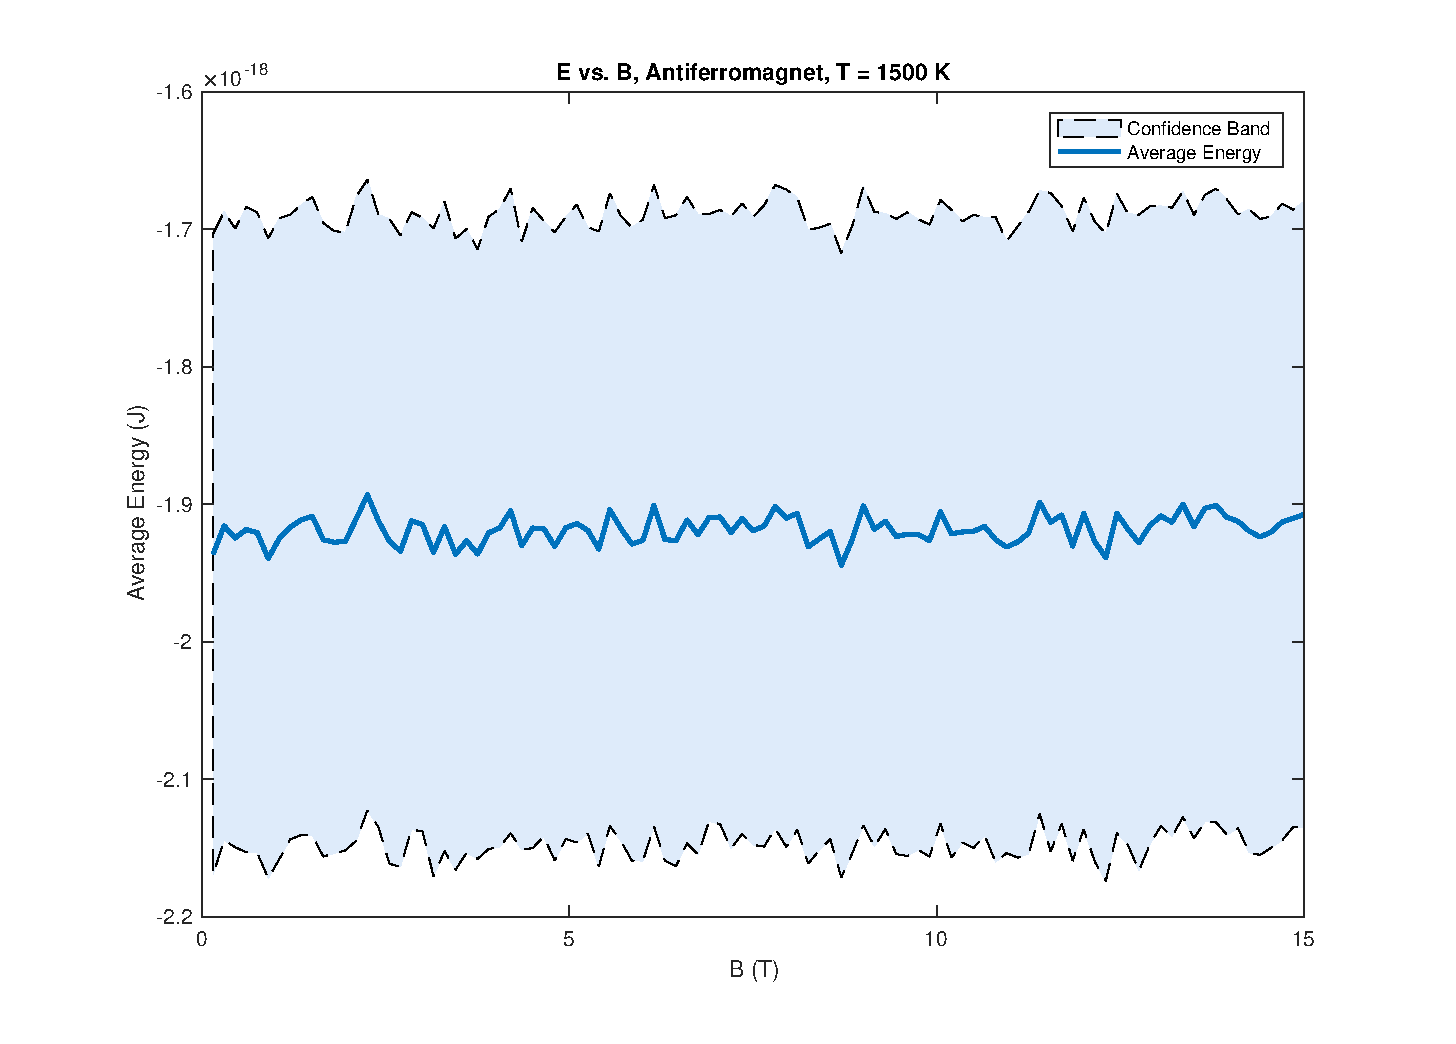
\includegraphics[width=\linewidth]{./Antiferrographs/antiferroEvsB.eps}
\caption{\label{antiferroEvsB}}
\end{subfigure}
\caption{Plots of (a) average magnetization as a function of applied magnetic field, and (b) average energy as a function of applied magnetic field.  These plots were produced using a temperature of $T$ = 1500 K.}  
\end{figure}
As we would expect at $T > T_N$, the antiferromagnetic behaves similar to a paramagnet as the magnetic field is increased.  In fig. \ref{antiferroMvsB} the linear relationship between magnetization and $B$ is quite clear.  The energy (fig. \ref{antiferroEvsB}) appears to vary marginally with magnetic field as $B$ increases, as expected due to its small contribution compared to the exchange forces.

\subsection*{Paramagnetism}
Past their threshold temperatures $T_N$ and $T_C$, both the ferromagnetic and antiferromagnetic materials behave as paramagnets.  This quality is characterized by no interaction between the neighboring spins in the lattice. \cite{magnettypes, fromjesse} Mathematically, in our Hamiltonian (eq. \ref{H}), $J=0$. \cite{magnettypes}

%Paramagnet 3D scatters
\begin{figure}[!h]
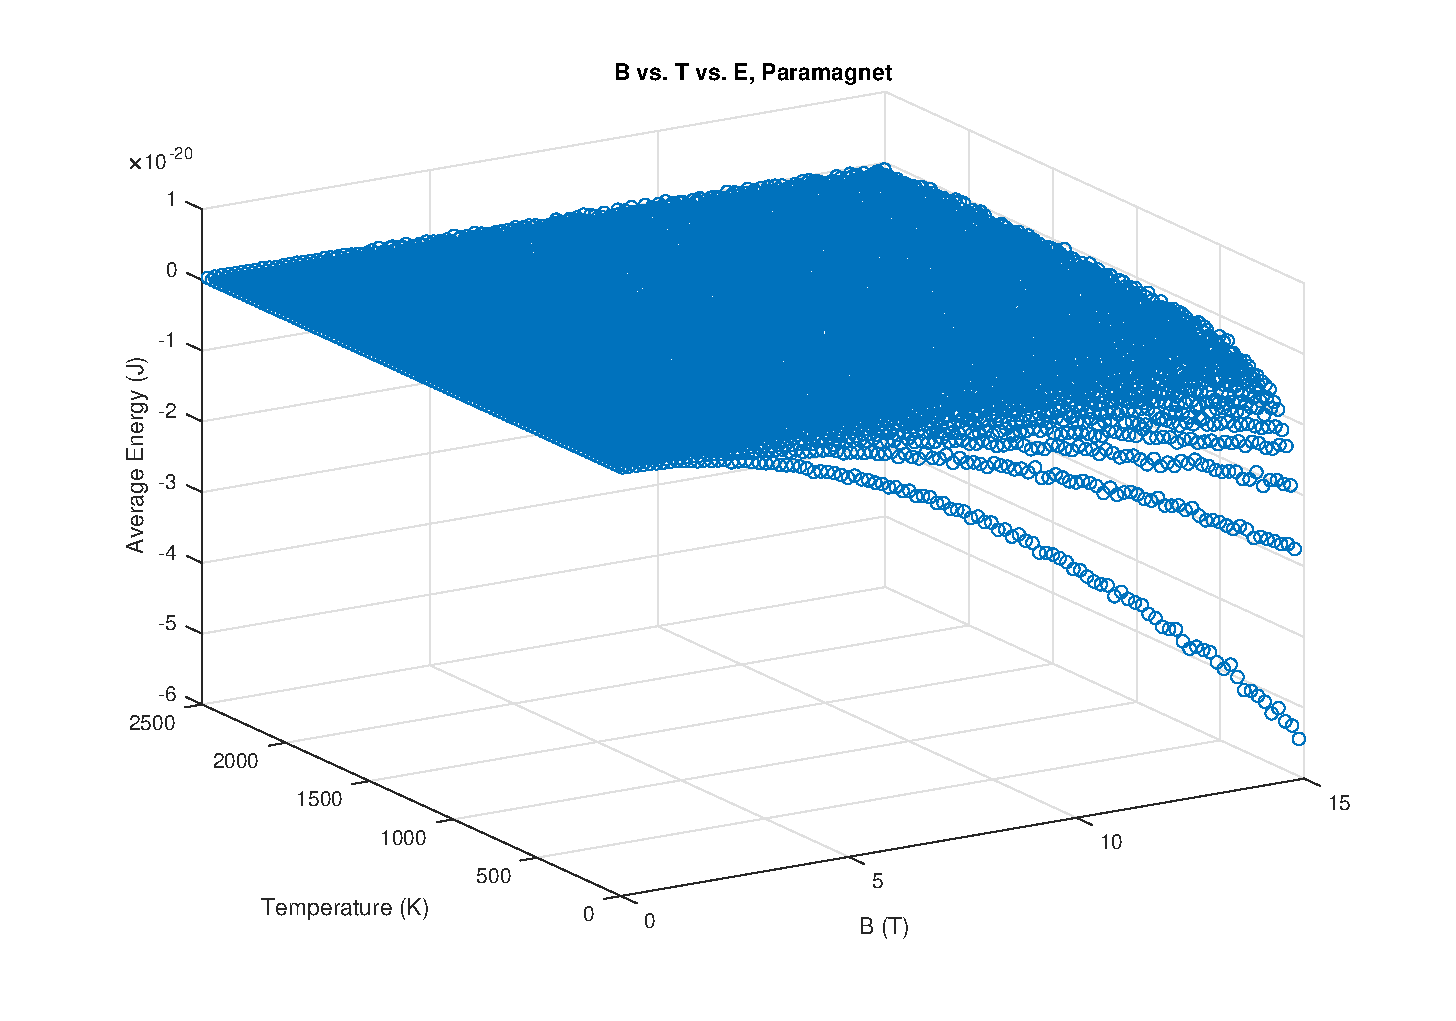
\includegraphics[width=\linewidth]{./Paragraphs/paraEsurf.eps}
\caption{A 3D scatter plot of average energy as a function of applied magnetic field $B$ and temperature.}
\label{paraEsurf}
\end{figure}
Because the energy in a paramagnetic is now completely dependent on the applied magnetic field multiplied by the spin states, the average energy is clearly zero for low $B$, evidenced in fig.\ref{paraEsurf}.  However, as the magnetic field increases, we see a drop off in average energy when at low enough temperature.

\begin{figure}[!h]
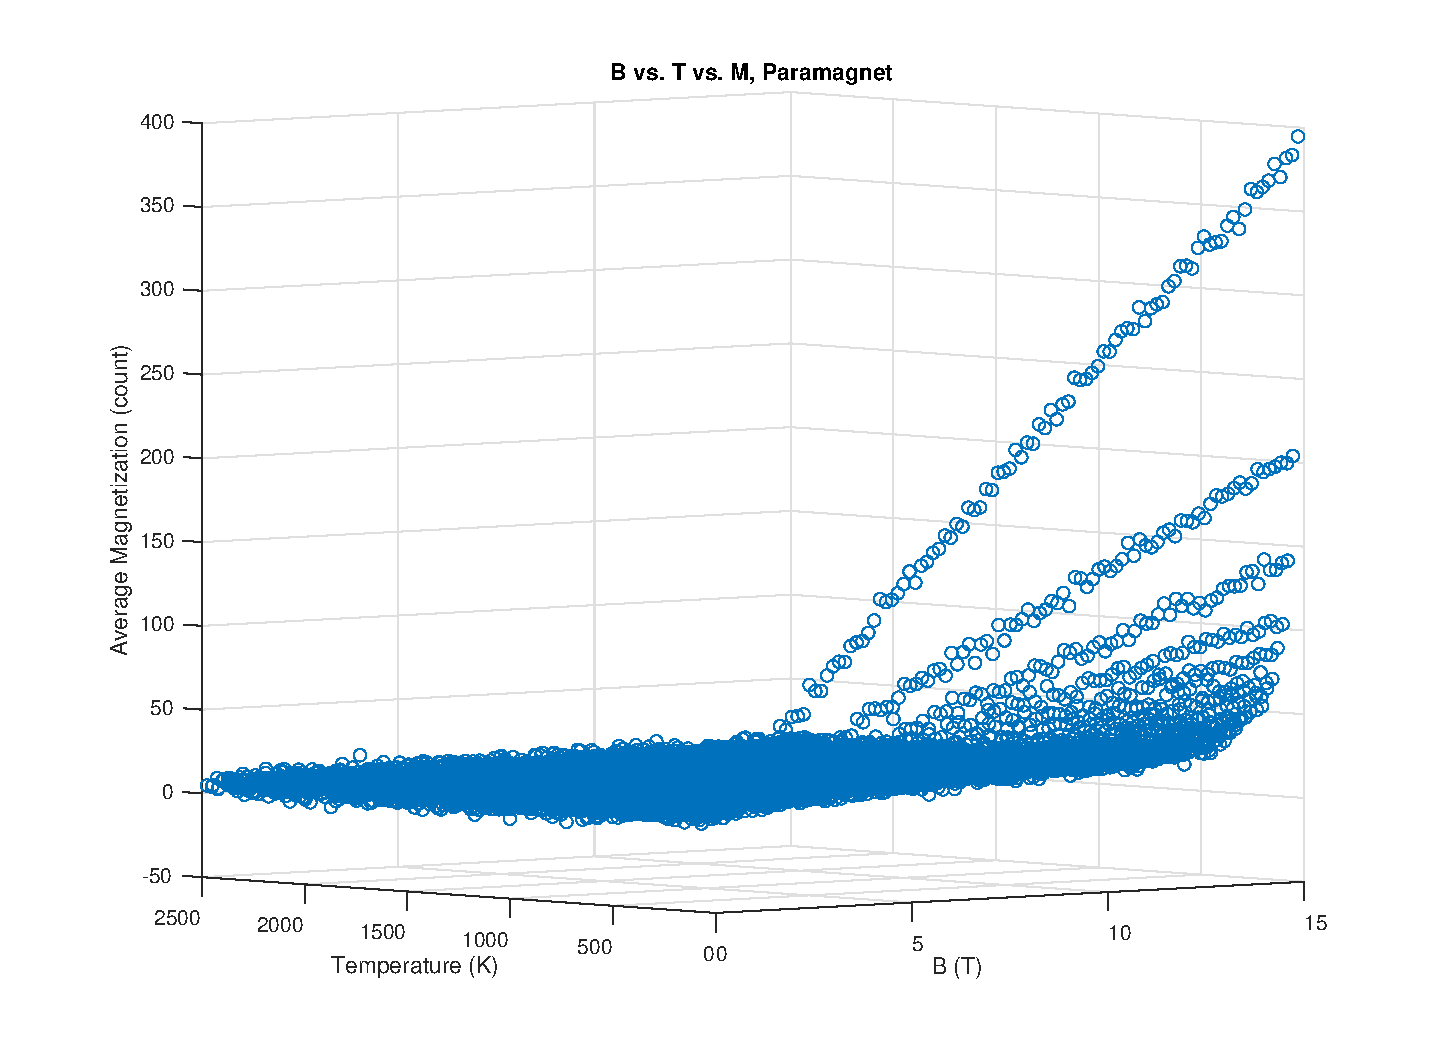
\includegraphics[width=\linewidth]{./Paragraphs/paraMsurf.eps}
\caption{A 3D scatter plot of average magnetization as a function of applied magnetic field $B$ and temperature $T$.}
\label{paraMsurf}
\end{figure}
The average magnetization now completely governs the energy of the system, so naturally fig. \ref{paraMsurf} is inversely related to the 3D scatter plot of energy shown in fig. \ref{paraEsurf}.  At low enough temperatures, the average magnetization increases linearly with $B$.

%Paramagnet T-dependent plots
\begin{figure}[!h]
\begin{subfigure}{0.5\textwidth}
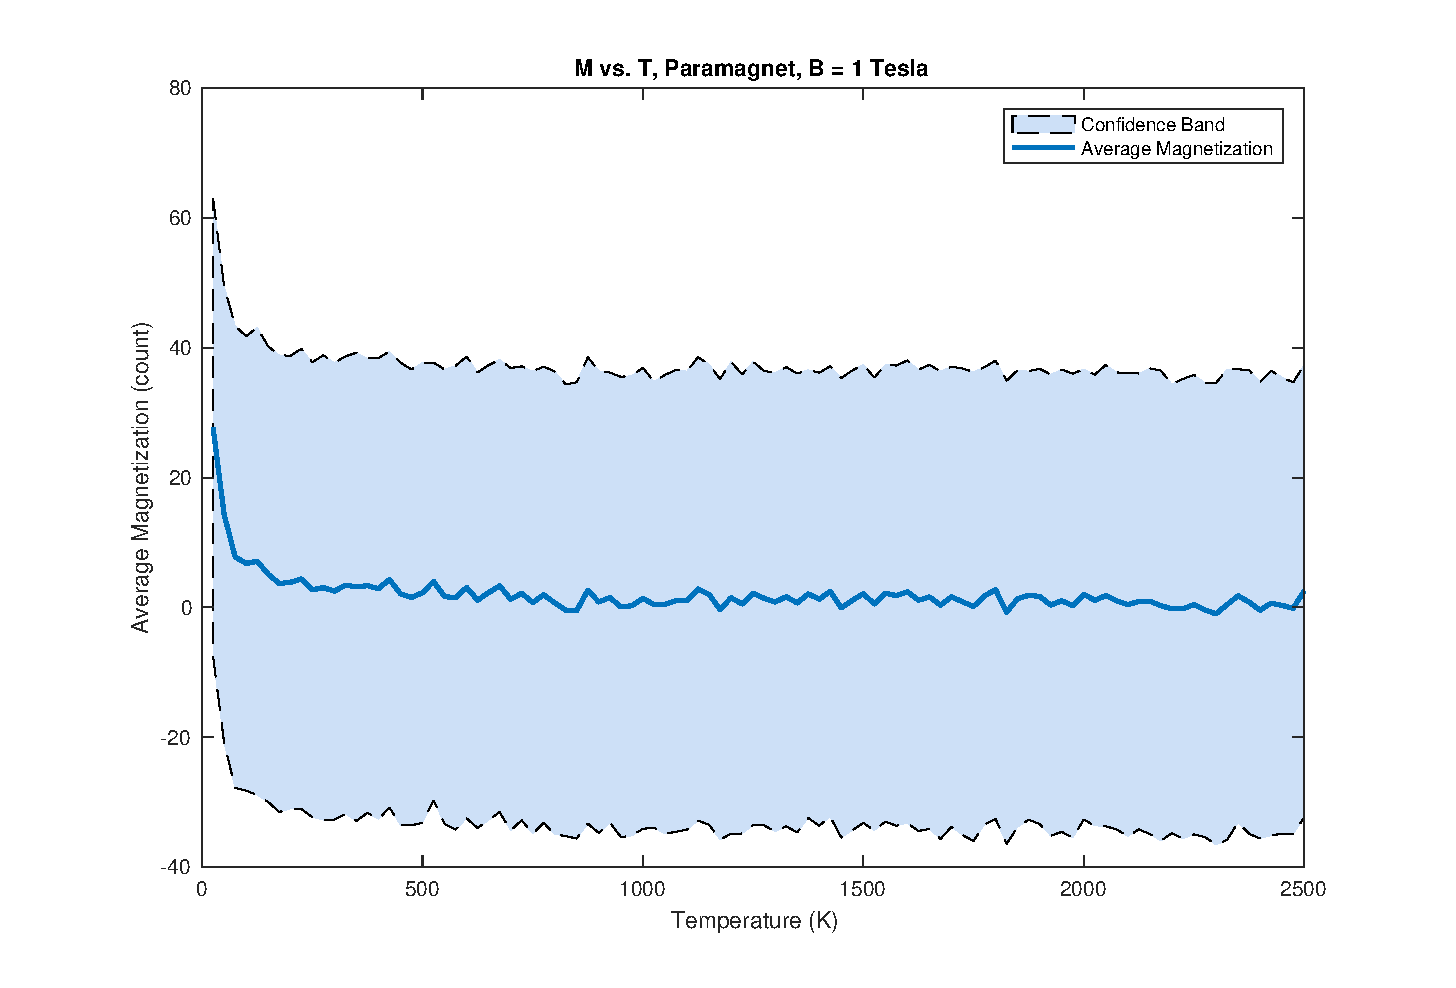
\includegraphics[width=\linewidth]{./Paragraphs/paraMvsT.eps}
\caption{\label{paraMvsT}}
\end{subfigure}
\begin{subfigure}{0.5\textwidth}
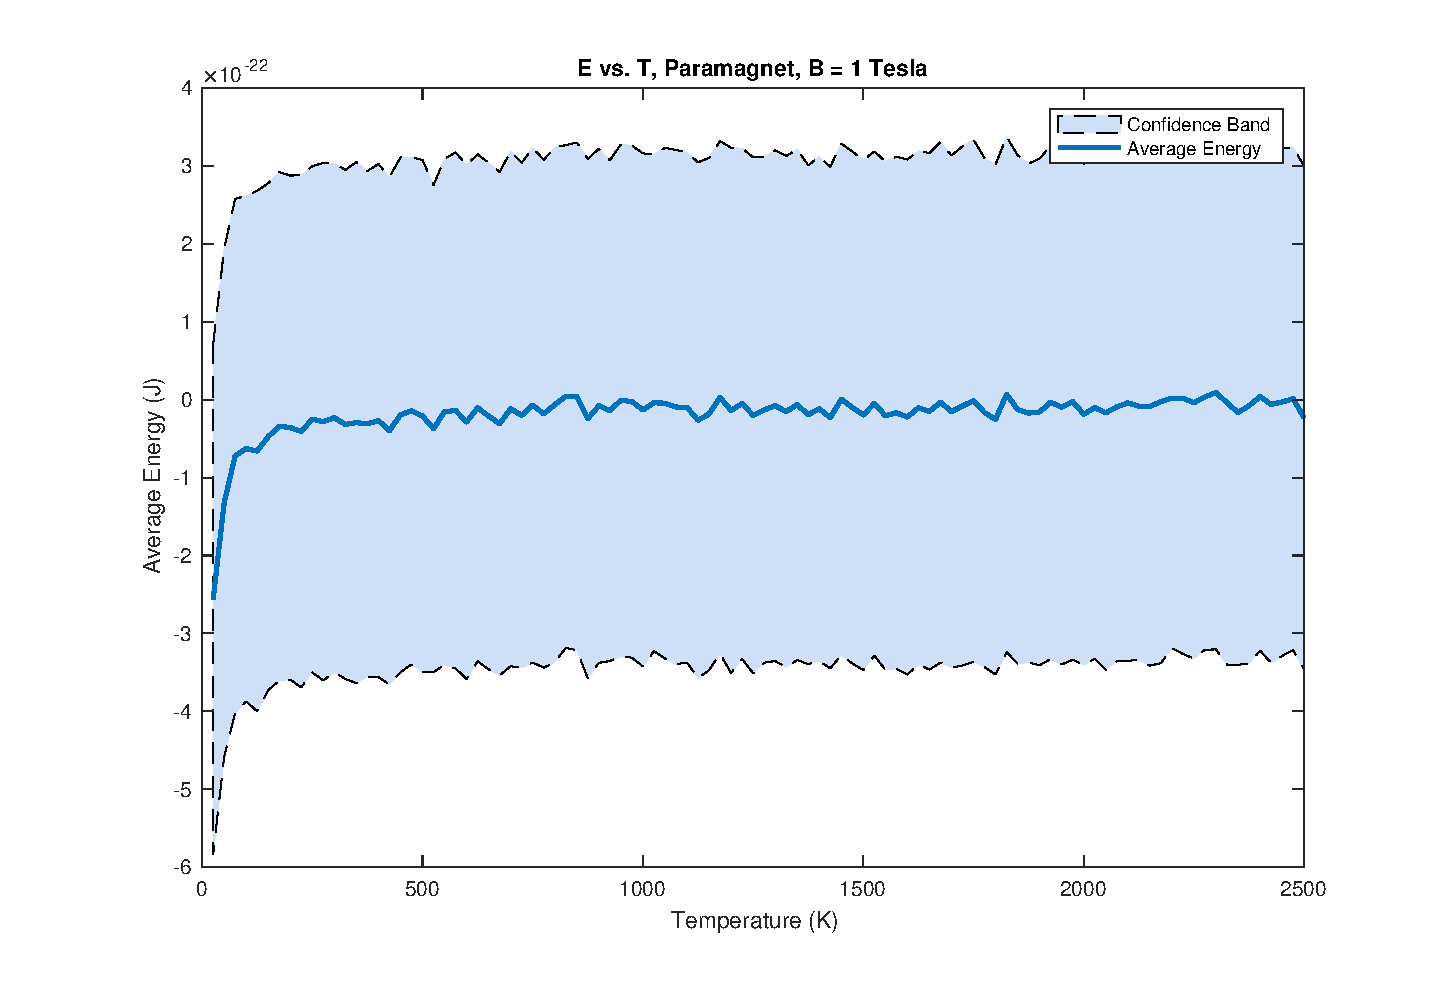
\includegraphics[width=\linewidth]{./Paragraphs/paraEvsT.eps}
\caption{\label{paraEvsT}}
\end{subfigure}
\caption{Plots of (a) average magnetization as a function of temperature, and (b) average energy as a function of temperature.  These plots were produced using an applied magnetic field $B$ = 1 T.} 
\end{figure} 
The graphs in figs. \ref{paraMvsT} and \ref{paraEvsT} further reiterate the concept that at low temperatures, there is not enough thermal energy in the system to overcome the influence of the magnetic field $B$.  As the temperature increases, the average magnetic moment also shifts to zero, and with it the average energy.

%Paramagnet B-dependent plots
\begin{figure}[!h]
\begin{subfigure}{0.5\textwidth}
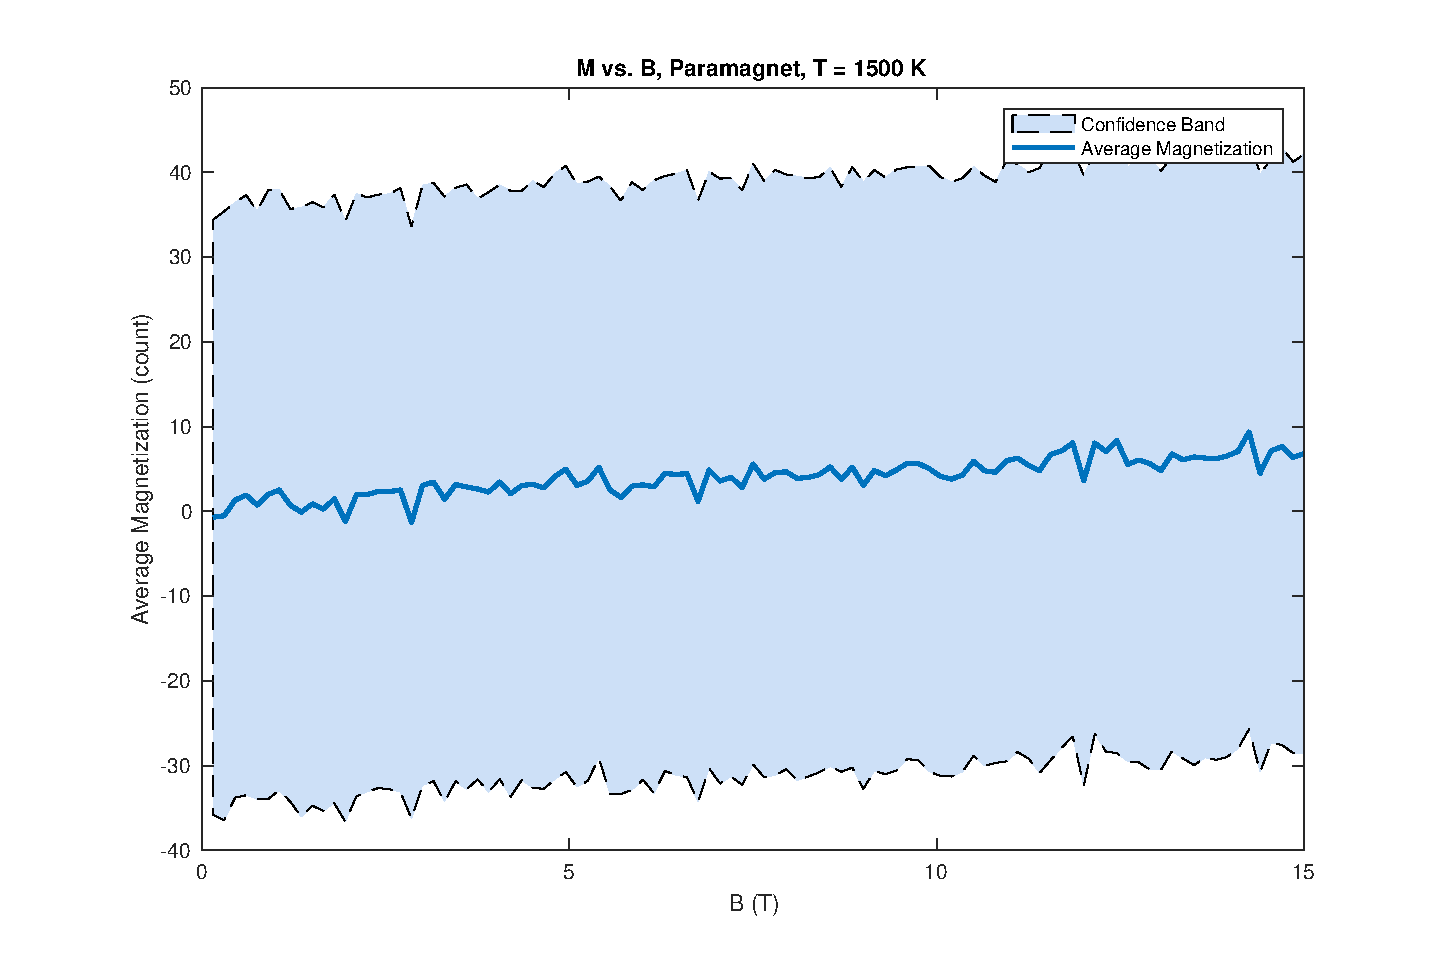
\includegraphics[width=\linewidth]{./Paragraphs/paraMvsB.eps}
\caption{\label{paraMvsB}}
\end{subfigure}
\begin{subfigure}{0.5\textwidth}
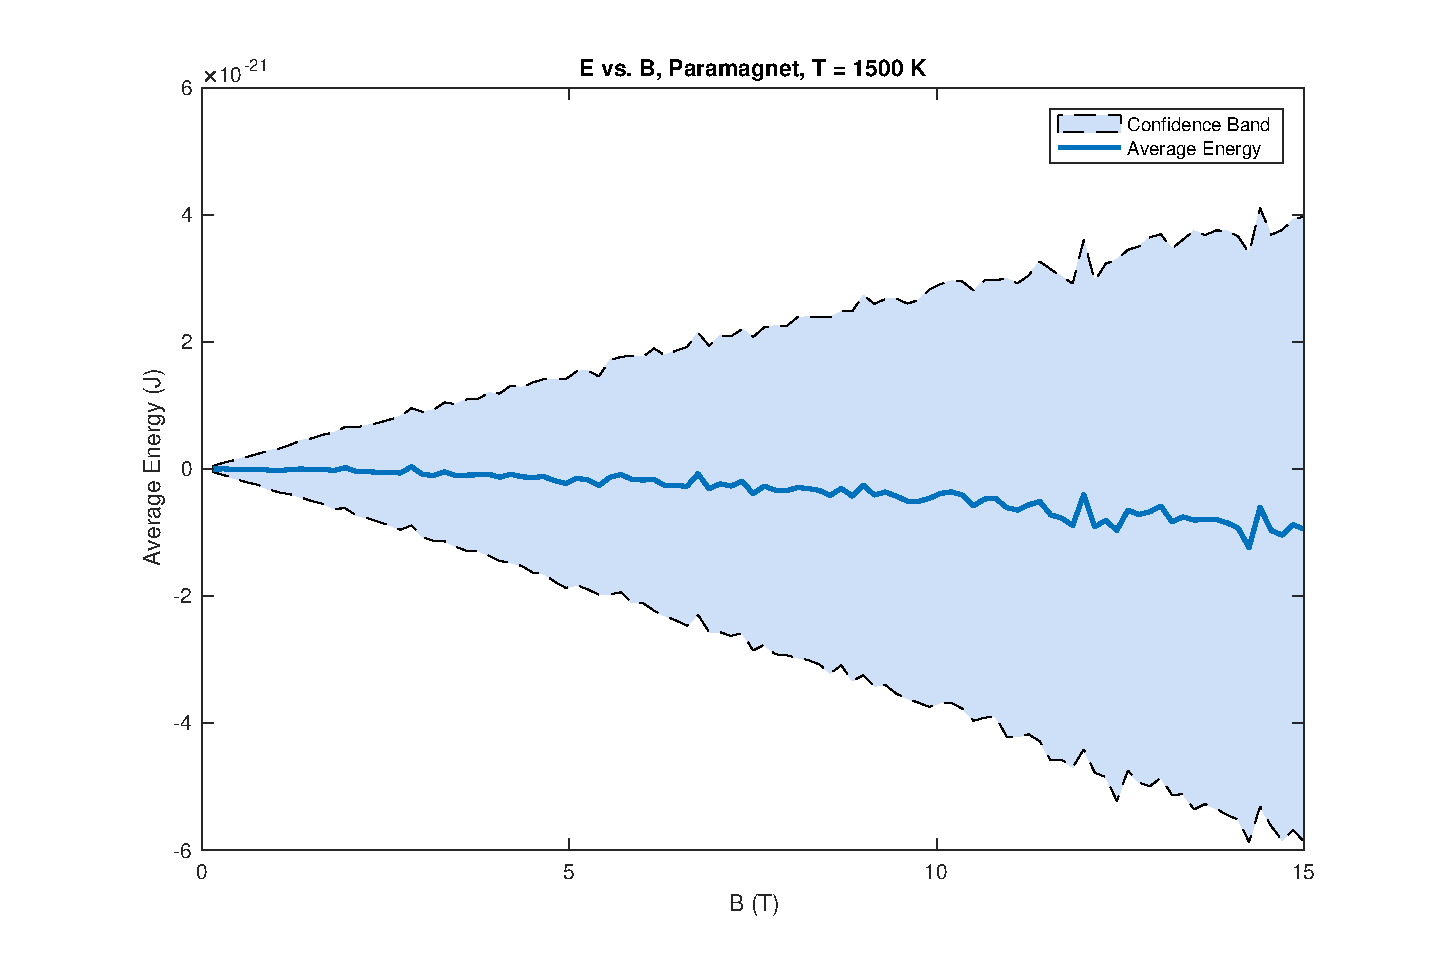
\includegraphics[width=\linewidth]{./Paragraphs/paraEvsB.eps}
\caption{\label{paraEvsB}}
\end{subfigure}
\caption{Plots of (a) average magnetization as a function of applied magnetic field, and (b) average energy as a function of applied magnetic field.  These plots were produced using a temperature of $T$ = 1500 K.}  
\end{figure}

\subsection*{Confidence Bands}
The confidence bands for the data tend to spread wider for larger temperature.  This stands to reason based on the At low temperatures, the energy and magnetization values accepted by the Monte-Carlo algorithm are all roughly the same energy, as there is not enough energy for the system to make large energy transitions.  As temperature increases, algorithm accepts more samples from a wider distribution, resulting in a higher standard deviation.

\subsection*{Discussion}
The Metropolis Monte Carlo algorithm simulates various magnetic materials with high precision and produces an accurate representation of the correlation between macroscopic values with microscopic effects.  These simulations identify both the approximate Curie temperature for ferromagnetic materials ($T_C \approx 1000$ K), and the N\'{e}el temperature for antiferromagnetic materials ($T_N \approx 75$ K.  As the temperature of the material rises above these exchange-interaction dependent temperatures, the material behavior transitions to paramagnetic, or an ``ideal" magnetic case.  In paramagnetic materials, it is clear the average magnetization depends linearly on the applied magnetic field, causing a decrease in average energy.

The simplicity and power of the Metropolis Monte Carlo algorithm is clear here--it allows for effective sampling based on simple acceptance and rejection criteria, in this case a probability distribution.  This algorithm lends itself easily to a variety of applications throughout computational physics and mathematics.

\newpage
\section*{Acknowledgements}
I would like to thank Dr. Justin Oelgoetz for assistance formulating the simulation code, and for providing insightful explanations and troubleshooting along the way.

The ``random\_number" subroutine within the code was seeded using an algorithm provided by Justin Oelgoetz, as sourced from open source code online.  This code seeds Fortran's random number generator to produce a more pseudo-random set of numbers that is unique to each run.

All graphs and plots made in this paper were produced using MATLAB computational software.
\newpage
\section*{Appendix}
Attached is the source code for this project, written in Fortran.
\lstinputlisting[language=Fortran]{../isingmodel.f90}
%Uncomment this shit for a bibliography
\newpage
\bibliographystyle{plain}
\bibliography{ising}
\end{document}